%%%%%%%%%%%%%%%%%%%% author.tex %%%%%%%%%%%%%%%%%%%%%%%%%%%%%%%%%%%
%
% sample root file for your "contribution" to a contributed volume
%
% Use this file as a template for your own input.
%
%%%%%%%%%%%%%%%% Springer %%%%%%%%%%%%%%%%%%%%%%%%%%%%%%%%%%


% RECOMMENDED %%%%%%%%%%%%%%%%%%%%%%%%%%%%%%%%%%%%%%%%%%%%%%%%%%%
\documentclass[graybox]{svmult}

\usepackage[utf8]{inputenc}
\usepackage{multirow}

% choose options for [] as required from the list
% in the Reference Guide

\usepackage{type1cm}        % activate if the above 3 fonts are
                            % not available on your system
%
\usepackage{makeidx}         % allows index generation
\usepackage{graphicx}        % standard LaTeX graphics tool
                             % when including figure files
\usepackage{multicol}        % used for the two-column index
\usepackage[bottom]{footmisc}% places footnotes at page bottom


\usepackage{newtxtext}       % 
\usepackage{newtxmath}       % selects Times Roman as basic font

% see the list of further useful packages
% in the Reference Guide

\makeindex             % used for the subject index
                       % please use the style svind.ist with
                       % your makeindex program

%%%%%%%%%%%%%%%%%%%%%%%%%%%%%%%%%%%%%%%%%%%%%%%%%%%%%%%%%%%%%%%%%%%%%%%%%%%%%%%%%%%%%%%%%

\begin{document}

\title*{Behavioral Analysis of Fuzzy Cognitive Maps}
% Use \titlerunning{Short Title} for an abbreviated version of
% your contribution title if the original one is too long
\author{Miklós F. Hatwagner}
% Use \authorrunning{Short Title} for an abbreviated version of
% your contribution title if the original one is too long
\institute{Miklós F. Hatwagner \at Széchenyi István University, Győr, 
Hungary \email{miklos.hatwagner@sze.hu}}
%
% Use the package "url.sty" to avoid
% problems with special characters
% used in your e-mail or web address
%
\maketitle

\newcommand{\behaviorAbstract}{Fuzzy Cognitive Maps are widely used in decision making. If 
historical time series data is available, the preferred way of model 
creation is based on machine learning. Sometimes such data in 
unavailable, however, and only experts can define the model. These 
models unavoidably contain more or less subjective elements, but 
even if the models are created by machine learning, their thorough 
investigation is recommended before usage. Sometimes a subtle 
modification of connection weights or a different $\lambda$ parameter 
in the threshold function can result in a model that behaves 
significatly different. This chapter describes a method to 
automatically investigate a model and detect if some of its components 
affect its dynamic hahavior significantly.}

\abstract*{\behaviorAbstract}

\abstract{\behaviorAbstract}

\section{Introduction}
\label{sec:intro}

Decision support systems and methods are at the center of 
researcher's attention for a long time \cite{busemeyer1999dynamic}, 
because prudent decision making can be really hard in practice, 
especially if the effect of many related factors with continuously 
changing states have to be taken into account, and a wrong 
intervention may cause serious personal injury or damage to property.

Chapter 1 gives an overview of Fuzzy Cognitive Maps (FCMs) \cite{b.kosko1986}, but it worth summarize the most important properties of FCMs again. FCM can be one of the possible tools of a decision-maker \cite{papageorgiou2013fuzzy}. 
It is a bipolar fuzzy graph that is made of nodes interconnected by directed, weighted edges. The various factors, variables of a 
complex system can be described by the nodes (also called \emph
{concepts}) and the strength of causal relations among them can be 
expressed by edges. Even if an FCM model can characterize the 
studied system only qualitatively \cite{j.l.salmeron2009}, this 
method is easy to use and provides a transparent, clear description 
of it. Modeling capabilities and simulations that reveal the dynamic 
behavior of the system made FCM an inevitable opportunity in 
decision support.

There are two main ways of model creation \cite{papageorgiou2012learning}:
\begin{enumerate}
  \item an expert, or a group of experts can give the description of 
  the system, or
  \item based on a long time-series database a suitable machine 
  learning technique may generate the model with more or less support 
  of experts.
\end{enumerate}

In the first case the expert who makes the model unavoidably 
includes his/her beliefs and subjectivity in the map. This can be 
decreased if a group of experts works out the model instead of a 
sole expert \cite{kosko1988hidden,groumpos2010fuzzy}, but the result 
will contain some uncertainty for sure. They can agree relatively 
quickly and easily on the number of concepts, the existence and sign 
of relationships, but the magnitude of those relationships are much 
harder to define, especially if an order of importance or strength 
exists among them. The number of relationships is a quadratic 
function of the number of concepts, therefore even if the modelers 
follow Kosko's advice and they do not include self-loops in the FCM, 
in case of a small model containing only 10 concepts the number of 
relationships can be up to 90. It will be really hard to define so 
many weights properly and worse is that the steepness parameter 
$\lambda$ of the threshold function does not have any connection 
with real objects, but its value may strongly influence the results 
of simulations (number and values of fixed points (FPs), limit cycles 
(LSs), chaotic behavior (CB)). FPs represent the stable states of a system and some of them should be achieved, others avoid according to the needs of stakeholders. LCs and CB are usually undesirable in decision making tasks.

Because of the inherent subjectivity and uncertainty the second method, based on machine learning is preferred 
in most cases of modeling. In those cases it can be applied the concepts 
are still defined by experts, however, and/or the nature of time series data. 
Sometimes such data is not available and only the first method 
remains.

Another possible scenario is when the model is created by the reduction of a bigger initial model (see Chapter 6). The reduction may cause smaller or larger behavioral changes according to the degree of reduction, eg. the number of fixed-point attractors can be different.

No matter how the model is made, it worth investigating the effect 
of small modifications of connection weights or steepness parameter 
on model behavior. The sensitive points of the model can be revealed 
and experts can discuss about the possibilities on making the model 
more stable and reliable. Unfortunately it cannot be made by hand, 
following a trial and error approach. In an FCM the connection 
weights are specified by real numbers, thus the number of possible 
modified weights are practically infinite. With a reasonable 
compromise we can say that the weights to try can be limited to the 
number of used linguistic variables, eg. 5: -1, -0.5, 0, 0.5 and 1. 
In the already mentioned model containing only 10 concepts, where 
even 90 relationships may exist, the number of model versions may up 
to $5^{90} = 8,078\times10^{62}$. Obviously the experts are primarily 
interested only in the effect of slight modifications, thus they 
would be satisfied with the check of one less and one greater values 
(or keeping the current one), but it could still mean $3^{90} = 
8,728\times10^{42}$ model versions. That can be even worse if they 
want to take the effect of different $\lambda$ values into account and 
of course, one simulation is not enough to characterize the behavioral 
effect of a modification, many simulations (depending on the model 
size to cover all interesting parts of the search space) are needed 
and these simulations are rather time consuming on their own. There is 
a clear need for an automated, consistent method for such 
investigations, and the work on that started in 
\cite{hatwagner2016uncertainty,hatwagner2017behavioral} and further 
developed in \cite{hatwagner2019banking,hatwagner2018improved}. This 
task is too big even for a computer: an exhaustive search cannot be 
performed, but an evolutionary search technique, eg. the Bacterial 
Evolutionary Algorithm is able to guide the directions of search for a 
slightly modified model that behaves significantly different.

\section{Bacterial Evolutionary Algorithm}
\label{sec:bea}

The thorough description of Bacterial Evolutionary Algorithm (BEA) 
can be found eg. in \cite
{nawa1997study,nawa1998study,nawa1998bacterial,nawa1999fuzzy}, only 
a short summary is given here to prove the applicability and 
usefulness of this algorithm. BEA is an evolutionary algorithm and 
as such able to solve any non-linear, highly modal, high dimensional 
global optimization problems. Another advantage is that it uses only 
a few parameters to set by the researcher. Despite its efficiency, 
BEA has high computational demand. It can be speed up by parallel 
execution \cite{hatwagner2011parallel} or by a problem specific 
local search operator \cite{koczy2018enhanced}, converting BEA to 
Bacterial Memetic Algorithm.

BEA works with a collection of possible solutions, which is also called 
\emph{population}. The algorithm continuously improves the members of 
the population, which are also called \emph{bacteria}, because the 
method imitates the reproduction and evolution of bacteria in the 
nature. Two operators are used to achieve this goal: \emph{bacterial 
mutation} is responsible for the exploration of the search space, and 
\emph{gene transfer} exploits the genetic information stored in 
bacteria in order to create new, hopefully fitter, more viable 
bacteria. The algorithm uses these operators alternately until the 
termination criterion is fulfilled, eg. a specified fitness value is 
achieved, a predefined number of generations are generated, the 
convergence slowed down, etc. Usually the best bacterium of the 
last population is considered result.

Bacterial mutation develops all bacteria at the same time, 
independently from each other. First, some identical copies of a 
bacterium are created, they are the \emph{clones} of the original 
bacterium. Then every alleles of the clones are mutated, changed in 
random order. If any of these changes lead to a better objective 
value, the old allele is replaced by the new one in the original 
bacterium and in all the clones. This operator is elitist by its 
nature because it keeps the genetic information of the old bacterium 
if newer bacteria are less fit.

Gene transfer starts with the sort of bacteria according to their 
fitness values. The bacteria with better fitness go in the 
\emph{superior} set, the remaining bacteria are locked up in the 
\emph{inferior} set. Next, the operator selects a bacterium randomly 
from the superior set, and another one from the inferior set. At least 
one allele of the better bacterium is transferred to the worse 
bacterium. Then the modified bacterium have to be evaluated again, and 
if it has a better objective value, it has a chance to migrate into 
the superior set and pass on its genetic data to other bacteria during 
the consecutive gene transfers.

\section{Details of the behavior analysis}
\label{sec:behaviorAnalysis}

The goal of behavior analysis is to modify a model only slightly but 
causing significant impact on its behavior at the same time. This 
can be an increased number of FPs, the presence of new LCs or CB. If 
such modifications are possible, they have to be further analysed by 
experts before the model is applied in decision making.

The search for small but significant modifications are controlled by 
BEA. In order to decrease the search space and accelerate the 
process, only 9 of the possible different weight values were tried 
in the last, most advanced version of the method \cite
{hatwagner2018improved}, according to the applied linguistic 
variables ($-1, -0.75, -0.5, ..., +1$). In our experience, experts 
reliably recognize the lack of causal relationships, therefore zero 
weight connections were left untouched. It also helps to speed up the 
search process.

The bacteria of BEA encodes a possible, common $\lambda$ value in the 
$[0.1, 10]$ interval for all concepts, and all non-zero connection 
weights in a fixed order.

The behavioral properties of modified models were tested with several 
simulations started with different inital state vectors. Only 5 
activation values were used: 0, 0.25, 0.5, 0.75 and 1. 1000 unique 
scenarios were generated randomly, and the same set was used to test 
all modified models for comparability. The program was prepared to 
automatically detect FPs, and count the number of different 
initial state vectors that resulted in the same FP. The simulations 
were definitely stopped after 100 iterations. In most cases, FCM 
converge very quickly to a FP. In the rare remaining cases the program 
searched for repeating sequences of state vectors to detect LCs. If it 
was not successful, the outcome of the simulation was considered a CB. 

The state of a model was considered stable only if the state of all 
concepts were stable, viz. their values changed by at most 0.001 in 
the last five consecutive time steps. Unfortunately the stable 
states are not exactly the same in many cases due to rounding errors 
of floating point arithmetic or other issues. That is why the 
similar final states were clustered by K-Means algorithm \cite
{hartigan1979algorithm} and the cluster centers were considered the 
common, stable, final states. K-Means needs to know the number of 
clusters in advance, however. It was automatically estimated by gap 
statistics \cite{tibshirani2001estimating}.

Behavioral analysis is a multiobjective optimization problem. The 
sometimes conflicting goals were as follows:
\begin{enumerate}
  \item maximize the number of FPs,
  \item maximize the number of LCs,
  \item maximize the number of CBs,
  \item maximize the similarity of original and modified model 
  versions.
\end{enumerate}

\noindent The similarity of models was measured by Eq.~\ref{eq:difference}.

\begin{equation}
  \label{eq:difference}
  d = \sum_{i=1}^{N} \sum_{j=1}^{N} (o_{ij} - m_{ij})^2
\end{equation}

\noindent where $d$ is the difference of models, $N$ is the number of 
concepts, $o_{ij}$ is the weight of connection in the original, and 
$m_{ij}$ is the weight of connection in the modified weight matrix. 
The fitness values of bacteria were defined in a Pareto-optimal 
manner. The Pareto-front of all bacteria constituted the members of the 
set of bacteria with highest fitness value, the Pareto-front of the 
remaining bacteria were the members of the set of second best bacteria, 
and so on.

\section{Case studies}
\label{sec:banking}

A real life problem of a bank was chosen in \cite
{hatwagner2018improved,hatwagner2019banking} to demonstrate the 
usefulness and operability of the developed program. Our client was interested in the result of different possible decisions regarding the organizational structure and operation which can be defined by performing FCM simulations. 

The concepts of the model are collected and interpreted in Table~\ref{tab:OMcategories}, the causal relationships among concepts are given by Table~\ref{tab:OMconnectionMtx}. 

\begin{table}
\caption{Concept IDs, names and categories of the first investigated model.}
\label{tab:OMcategories}
\begin{center}
\begin{tabular}{lll}
\hline\noalign{\smallskip}
Concept ID & Concept name & Category\\
\noalign{\smallskip}\svhline\noalign{\smallskip}
C1 & Clients & \multirow{3}{*}{Assets}\\
C2 & Rules \& regulations & \\
C3 & New IT solutions & \\
\noalign{\smallskip} \hline \noalign{\smallskip}
C4 & Funding & \multirow{2}{*}{Money}\\
C5 & Cost reduction & \\
\noalign{\smallskip} \hline \noalign{\smallskip}
C6 & Profit/loss & \multirow{2}{*}{Financials}\\
C7 & Investments & \\
\noalign{\smallskip} \hline \noalign{\smallskip}
C8 & Staff & Human resources\\
\noalign{\smallskip} \hline \noalign{\smallskip}
C9 & New services & \multirow{2}{*}{Product and process development}\\
C10 & Quality & \\
\noalign{\smallskip} \hline \noalign{\smallskip}
C11 & Client development & \multirow{3}{*}{Output measures}\\
C12 & Service development & \\
C13 & Productivity & \\
\noalign{\smallskip} \hline
\end{tabular}
\end{center}
\end{table}

\begin{table}
\caption{Connection matrix of the first example FCM model.}
\label{tab:OMconnectionMtx}
\begin{center}
\begin{tabular}{l|lllllllllllll}
\hline\noalign{\smallskip}
 & C1 & C2 & C3 & C4 & C5 & C6 & C7 & C8 & C9 & C10 & C11 & C12 & C13\\
\noalign{\smallskip}\hline\noalign{\smallskip}
C1 &    0 &     0 &     0.5 &   0 &     0 &     0.5 &   1 &     0.5 &   0 &     0.5 &   1 &     0.5 &   0\\
C2 &    1 &     0 &     0.5 &   1 &     0 &     0 &     1 &     1 &     0.5 &   0 &     1 &     1 &     0\\
C3 &    1 &     0.5 &   0 &     0 &     0 &     -1 &    0 &     -1 &    1 &     0 &     1 &     1 &     1\\
C4 &    0 &     0 &     0 &     0 &     0 &     0 &     0 &     0 &     0 &     0 &     0 &     0 &     0\\
C5 &    0 &     0 &     1 &     -0.5 &  0 &     0 &     0 &     -1 &    0 &     0 &     0 &     1 &     0\\
C6 &    0 &     0 &     0 &     0 &     -0.5 &  0 &     0 &     0 &     0 &     0 &     0 &     0 &     0\\
C7 &    0.5 &   0 &     0.5 &   1 &     0 &     0.5 &   0 &     0 &     0 &     -0.5 &  0 &     0 &     0\\
C8 &    0 &     0 &     0 &     0 &     0 &     -0.5 &  0 &     0 &     0 &     0.5 &   0 &     0 &     -0.5\\
C9 &    0 &     0 &     0 &     1 &     0 &     0.5 &   0.5 &   0.5 &   0 &     -0.5 &  0 &     0.5 &   0\\
C10 &   0.5 &   0 &     0 &     0 &     0 &     0 &     0.5 &   0.5 &   0.5 &   0 &     1 &     0 &     0\\
C11 &   0 &     0 &     0.5 &   0.5 &   0 &     0 &     0 &     0 &     0.5 &   0.5 &   0 &     0 &     1\\
C12 &   0 &     0 &     0.5 &   0.5 &   0 &     0 &     1 &     0 &     0.5 &   0 &     0.5 &   0 &     -0.5\\
C13 &   0 &     0 &     1 &     0 &     0 &     0.5 &   0 &     0 &     0 &     0 &     1 &     0 &     0\\
\noalign{\smallskip}\hline
\end{tabular}
\end{center}
\end{table}

First, the behavior of the original model was analyzed. The $\lambda$ 
steepness parameter of the threshold function used in the inference 
equation was set to 5. Two FPs were found. 23.1\% of the investigated 
cases resulted in the first, and the remaining 76.9\% in the second 
FP. These FPs are pretty similar, only the values of concepts C6 and 
C8 differentiates them. C4 is an input concept and it was left out 
from Table~\ref{tab:OMFPs}. 

\begin{table}
\caption{Fixed-point attractors of the first example model.}
\label{tab:OMFPs}
\begin{center}
\begin{tabular}{llll}
\hline\noalign{\smallskip}
Concepts & C1-C3, C5, C7, C9-C13 & C6 & C8\\
\noalign{\smallskip}\svhline\noalign{\smallskip}
FP\#1 & 1.000 & 0.150 & 0.990\\
FP\#2 & 1.000 & 0.855 & 0.922\\
\noalign{\smallskip}\hline
\end{tabular}
\end{center}
\end{table}

The state represented by the second FP is much more desirable than the first, because it means that higher profit can be reached, while the number of staff can also be decreased. The result of every possible decisions can be checked by an FCM simulation.

The connection matrix was created by experts and may contain subjective elements and intrinsic uncertainty, however. It is hard to define the connection weight of all the 61 connections, even if only five weight values were used. If only some of these relations are estimated wrong, the result of a decision can be different than the predicted one and large financial loss may be suffered. Moreover, the value of the steepness parameter $\lambda$ was chosen according to its widely applied value in literature (5), but it does not have any relationship with the modeled system. What if using another value a significantly different state will be predicted? Before realizing any intervention in the life of the organisation it worth checking the consequences of the same decision with a slightly modified model. Maybe a bit higher or lover $\lambda$ value, a modified connection weight lead to a significantly different effect which must be further analysed and validated. If such a slightly modified model cannot be found, the developed model can be used with a higher degree of confidence.

The results of such an analysis are interesting even if the weights are  well-chosen, because if the behavior of these modified models are known it can be seen how and where should the model be changed in order to eventuate a better operation, or what effects jeopardize the operation of it.

That is why the behavioral analysis of modified models followed. The 
model contains 13 concepts, but the density of it is only $\approx$39
\%. It still meant a 62 variable optimization problem. The 
population of BEA consisted of 10 bacteria, 3 clones were created 
for each bacterium, and also 3 gene transfers were applied in the 
consecutive iterations. The optimization was stopped after the 10%
\textsuperscript{th} generation. The connection matrices of the two 
best modified models (they are the members of the first 
Pareto-front, see Fig.~\ref{fig:pareto}) are given by Tables~\ref
{tab:V1connectionMtx} and \ref{tab:V2connectionMtx}. The main 
properties of these models are collected in Table~\ref
{tab:variantsProps}. 

It is clear that with slight model modifications much more, over 40 possible outcomes can occur. It is vital to re-check the consequences of decisions which led to the same FP in the case of the original model.

\begin{figure}
  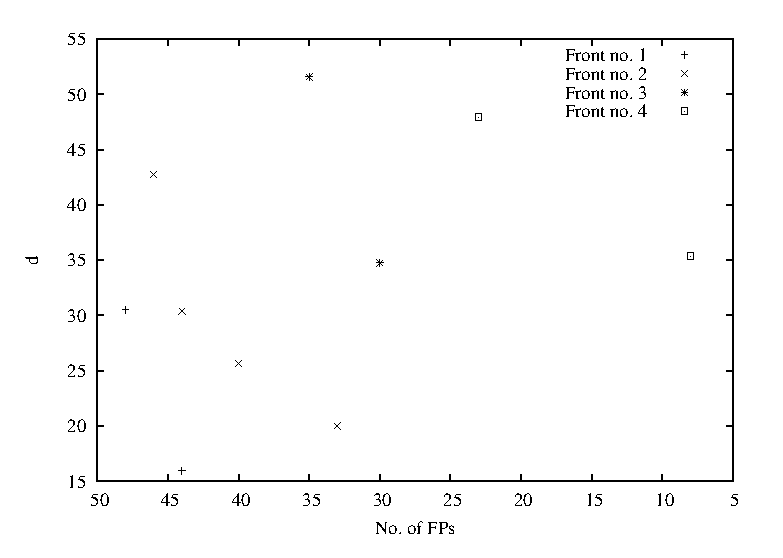
\includegraphics[width=\textwidth]{pareto.eps}
  \caption{Bacteria of Pareto-fronts in the last generation.}
  \label{fig:pareto}
\end{figure}

\begin{table}
\caption{Connection matrix of the 1\textsuperscript{st} model variant of the first example model.}
\label{tab:V1connectionMtx}
\begin{center}
\begin{tabular}{l|lllllllllllll}
\hline\noalign{\smallskip}
 &      C1 &    C2 &    C3 &    C4 &    C5 &    C6 &    C7 &    C8 &    C9 &    C10 &   C11 &   C12 &   C13\\
\noalign{\smallskip}\hline\noalign{\smallskip}
C1 &    0.0 &   0.0 &   0.75 &  0.0 &   0.0 &   0.5 &   1.0 &   0.25 &  0.0 &   0.25 &  0.75 &  0.5 &   0.0\\
C2 &    1.0 &   0.0 &   0.5 &   1.0 &   0.0 &   0.0 &   0.5 &   0.75 &  0.75 &  0.0 &   0.75 &  1.0 &   0.0\\
C3 &    0.25 &  0.0 &   0.0 &   0.0 &   0.0 &   -1.0 &  0.0 &   -0.75 & 0.5 &   0.0 &   0.5 &   0.75 &  1.0\\
C4 &    0.0 &   0.0 &   0.0 &   0.0 &   0.0 &   0.0 &   0.0 &   0.0 &   0.0 &   0.0 &   0.0 &   0.0 &   0.0\\
C5 &    0.0 &   0.0 &   1.0 &   -0.5 &  0.0 &   0.0 &   0.0 &   0.0 &   0.0 &   0.0 &   0.0 &   0.5 &   0.0\\
C6 &    0.0 &   0.0 &   0.0 &   0.0 &   -0.5 &  0.0 &   0.0 &   0.0 &   0.0 &   0.0 &   0.0 &   0.0 &   0.0\\
C7 &    0.75 &  0.0 &   -0.25 & 1.0 &   0.0 &   0.25 &  0.0 &   0.0 &   0.0 &   1.0 &   0.0 &   0.0 &   0.0\\
C8 &    0.0 &   0.0 &   0.0 &   0.0 &   0.0 &   0.25 &  0.0 &   0.0 &   0.0 &   0.75 &  0.0 &   0.0 &   -0.5\\
C9 &    0.0 &   0.0 &   0.0 &   1.0 &   0.0 &   0.25 &  -0.75 & 0.25 &  0.0 &   0.25 &  0.0 &   0.75 &  0.0\\
C10 &   -0.75 & 0.0 &   0.0 &   0.0 &   0.0 &   0.0 &   0.25 &  -0.5 &  0.25 &  0.0 &   -0.25 & 0.0 &   0.0\\
C11 &   0.0 &   0.0 &   0.75 &  0.5 &   0.0 &   0.0 &   0.0 &   0.0 &   0.5 &   0.5 &   0.0 &   0.0 &   1.0\\
C12 &   0.0 &   0.0 &   0.5 &   0.5 &   0.0 &   0.0 &   0.25 &  0.0 &   0.25 &  0.0 &   -0.75 & 0.0 &   -0.5\\
C13 &   0.0 &   0.0 &   0.75 &  0.0 &   0.0 &   0.75 &  0.0 &   0.0 &   0.0 &   0.0 &   0.75 &  0.0 &   0.0\\
\noalign{\smallskip}\hline
\end{tabular}
\end{center}
\end{table}

\begin{table}
\caption{Connection matrix of the 2\textsuperscript{nd} model variant of the first example model.}
\label{tab:V2connectionMtx}
\begin{center}
\begin{tabular}{l|lllllllllllll}
\hline\noalign{\smallskip}
 &      C1 &    C2 &    C3 &    C4 &    C5 &    C6 &    C7 &    C8 &    C9 &    C10 &   C11 &   C12 &   C13\\
\noalign{\smallskip}\hline\noalign{\smallskip}
C1 &    0.0 &   0.0 &   0.5 &   0.0 &   0.0 &   0.5 &   1.0 &   1.0 &   0.0 &   1.0 &   0.75 &  0.5 &   0.0\\
C2 &    -0.75 & 0.0 &   0.0 &   1.0 &   0.0 &   0.0 &   0.5 &   0.0 &   0.5 &   0.0 &   0.0 &   0.5 &   0.0\\
C3 &    0.25 &  0.25 &  0.0 &   0.0 &   0.0 &   -0.75 & 0.0 &   -1.0 &  0.0 &   0.0 &   0.5 &   -0.5 &  0.0\\
C4 &    0.0 &   0.0 &   0.0 &   0.0 &   0.0 &   0.0 &   0.0 &   0.0 &   0.0 &   0.0 &   0.0 &   0.0 &   0.0\\
C5 &    0.0 &   0.0 &   -0.5 &  -0.5 &  0.0 &   0.0 &   0.0 &   0.25 &  0.0 &   0.0 &   0.0 &   0.5 &   0.0\\
C6 &    0.0 &   0.0 &   0.0 &   0.0 &   0.0 &   0.0 &   0.0 &   0.0 &   0.0 &   0.0 &   0.0 &   0.0 &   0.0\\
C7 &    0.5 &   0.0 &   0.0 &   1.0 &   0.0 &   0.75 &  0.0 &   0.0 &   0.0 &   -0.5 &  0.0 &   0.0 &   0.0\\
C8 &    0.0 &   0.0 &   0.0 &   0.0 &   0.0 &   -1.0 &  0.0 &   0.0 &   0.0 &   1.0 &   0.0 &   0.0 &   0.5\\
C9 &    0.0 &   0.0 &   0.0 &   1.0 &   0.0 &   0.0 &   0.75 &  1.0 &   0.0 &   -0.75 & 0.0 &   0.75 &  0.0\\
C10 &   0.5 &   0.0 &   0.0 &   0.0 &   0.0 &   0.0 &   0.0 &   0.5 &   -0.25 & 0.0 &   -0.75 & 0.0 &   0.0\\
C11 &   0.0 &   0.0 &   -1.0 &  0.5 &   0.0 &   0.0 &   0.0 &   0.0 &   0.25 &  1.0 &   0.0 &   0.0 &   -1.0\\
C12 &   0.0 &   0.0 &   0.0 &   0.5 &   0.0 &   0.0 &   1.0 &   0.0 &   0.5 &   0.0 &   -0.25 & 0.0 &   0.25\\
C13 &   0.0 &   0.0 &   1.0 &   0.0 &   0.0 &   0.75 &  0.0 &   0.0 &   0.0 &   0.0 &   0.5 &   0.0 &   0.0\\
\noalign{\smallskip}\hline
\end{tabular}
\end{center}
\end{table}

\begin{table}
\caption{Main properties of the modified model variants on Pareto front \#1.}
\label{tab:variantsProps}
\begin{center}
\begin{tabular}{lll}
\hline\noalign{\smallskip}
Property & 1\textsuperscript{st} variant & 2\textsuperscript{nd} variant\\
\noalign{\smallskip}\svhline\noalign{\smallskip}
$\lambda$ value & 2.366 & 2.070 \\
Number of FPs & 44 & 48 \\
Number of LCs & 0 & 0 \\
Number of chaotic behavior & 0 & 0 \\
Difference from orig. model ($d$) & 15.938 & 30.500 \\
\noalign{\smallskip}\hline
\end{tabular}
\end{center}
\end{table}

As a second example, another model of the same bank is presented (see Table~\ref{tab:BP2Spartial-connectionMtx} and Fig.~\ref{fig:BP2Spartial}). Due to the confidential nature of the data, the meaning of concepts and their connections cannot be detailed here, but this is not relevant to the presentation of the applied method, neither. The behavior of the model was analysed using three different $\lambda$ values first, without any modifications on the connection matrix. When the steepness parameter was set to 5, three FPs were found (see Table~\ref{tab:BP2Spartial5-FPs}). The last one occurred only in 0.2\% of the investigated cases. This raises the suspicion that this is not a real fixed point, but an extremely slow convergence to another fixed point happened, which was mistakenly perceived by the software as a FP. However, repeating the study with a reduced $\lambda$ value of 4.7, it can be seen that the incidence of the same fixed point increased to 8.2\%, while the activation value of concept C2.5 left practically the same (0.506 vs. 0.502). Even some inital state vectors are listed in Table~\ref{tab:BP2Spartial-scenarios} as examples that lead to the specified FPs. Further reducing the value of the $\lambda$ parameter to 1.4235, only one fixed point remained (see Table~\ref{tab:BP2Spartial14235-FPs}). These examinations show how important the value of parameter $\lambda$ is in FCM simulations. The effect of any planned interventions must be checked by several simulations using various steepness parameters in order to realize all the possible outcomes.

\begin{table}
\caption{Connection matrix of the second example FCM model.}
\label{tab:BP2Spartial-connectionMtx}
\begin{center}
\begin{tabular}{l|lllllllllll}
\hline\noalign{\smallskip}
 & C1.2 & C2.4 & C2.5 & C3.1 & C3.2 & C4.1 & C5.2 & C5.3 & C6.1 & C6.2 & C6.3\\
\noalign{\smallskip}\hline\noalign{\smallskip}
C1.2 & 0 & 0 & 0 & 0.5 & 1 & 0.5 & 0 & 0.5 & 1 & 0.5 & 0\\
C2.4 & 0 & 0 & 0 & 0 & 0 & 0 & 0 & 0 & 0 & 0 & 0\\
C2.5 & 0 & -0.5 & 0 & 0 & 0 & -1 & 0 & 0 & 0 & 1 & 0\\
C3.1 & 0 & 0 & -0.5 & 0 & 0 & 0 & 0 & 0 & 0 & 0 & 0\\
C3.2 & 0.5 & 1 & 0 & 0.5 & 0 & 0 & 0 & -0.5 & 0 & 0 & 0\\
C4.1 & 0 & 0 & 0 & -0.5 & 0 & 0 & 0 & 0.5 & 0 & 0 & -0.5\\
C5.2 & 0 & 1 & 0 & 0.5 & 0.5 & 0.5 & 0 & -0.5 & 0 & 0.5 & 0\\
C5.3 & 0.5 & 0 & 0 & 0 & 0.5 & 0.5 & 0.5 & 0 & 1 & 0 & 0\\
C6.1 & 0 & 0.5 & 0 & 0 & 0.5 & 0 & 0.5 & 0.5 & 0 & 1 & 1\\
C6.2 & 0 & 0.5 & 0 & 0 & 1 & 0 & 0.5 & 0 & 0.5 & 0 & -0.5\\
C6.3 & 0 & 0 & 0 & 0.5 & 0 & 0 & 0 & 0 & 1 & 0 & 0\\
\noalign{\smallskip}\hline
\end{tabular}
\end{center}
\end{table}

\begin{figure}
  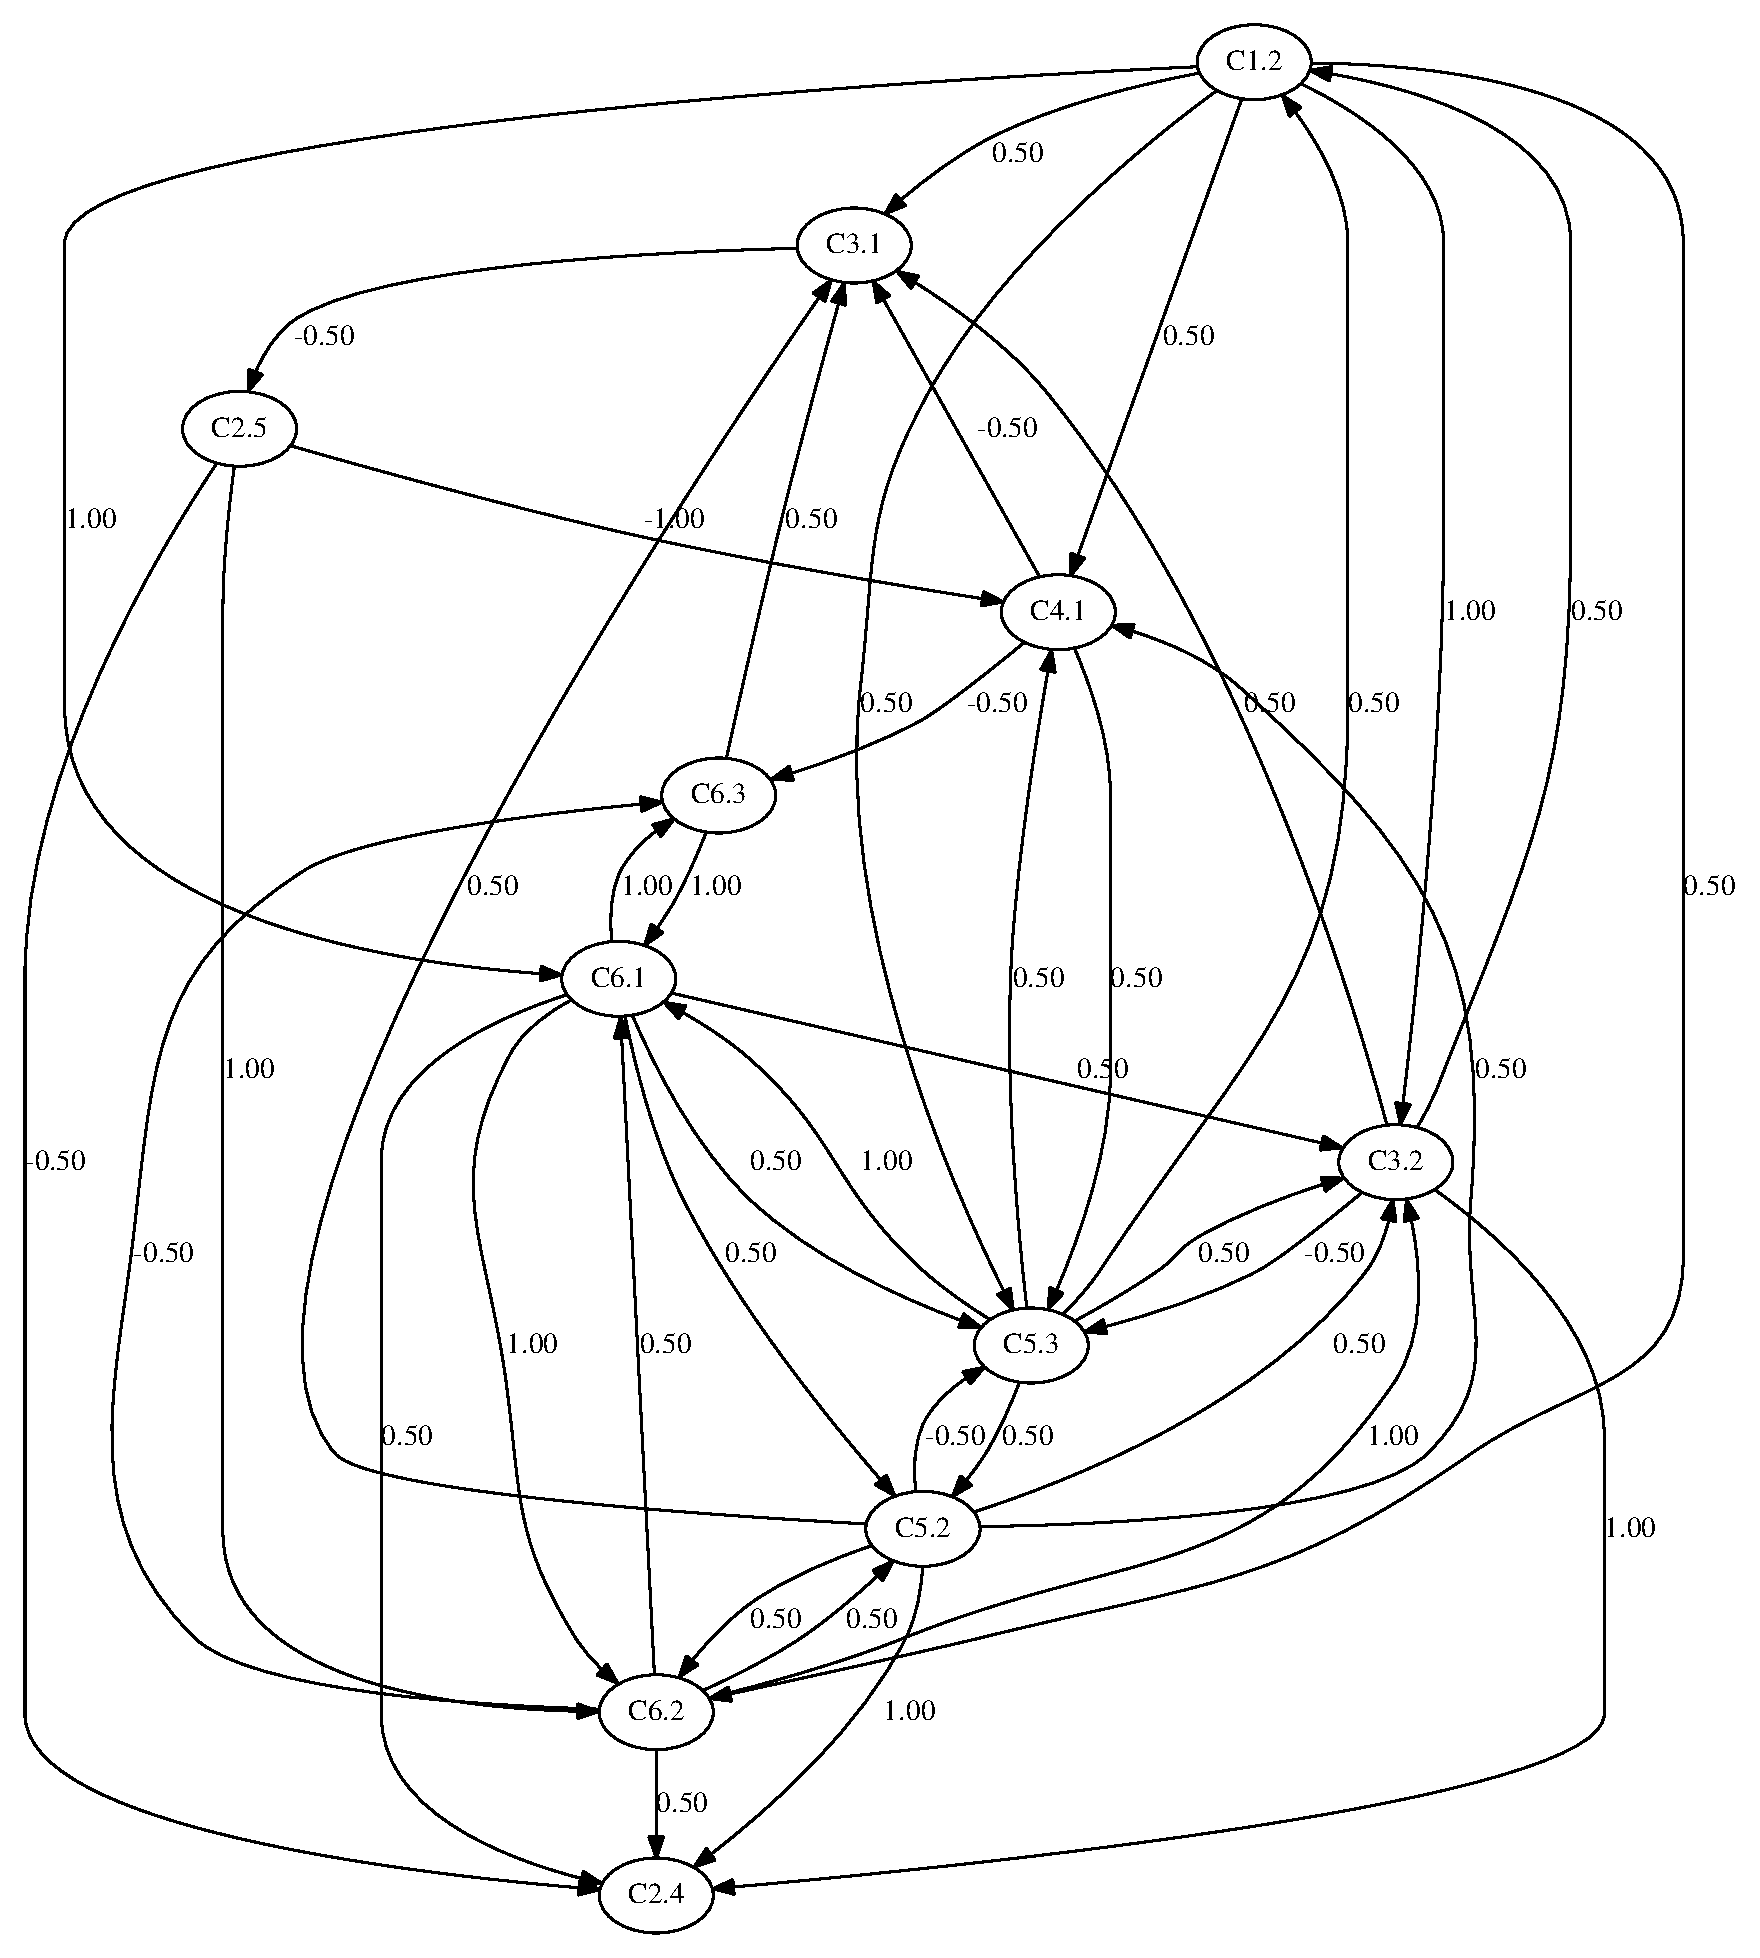
\includegraphics[width=\textwidth]{BP2Spartial.eps}
  \caption{Graph representation of the second example model.}
  \label{fig:BP2Spartial}
\end{figure}

\begin{table}
\caption{Fixed-point attractors of the second example model ($\lambda = 5$).}
\label{tab:BP2Spartial5-FPs}
\begin{center}
\begin{tabular}{lllllll}
\hline\noalign{\smallskip}
Concepts & C1.2, C2.4 & C2.5 & C3.1, C3.2, C4.1, C5.2 & C5.3 & C6.1, C6.2 & C6.3\\
\noalign{\smallskip}\svhline\noalign{\smallskip}
FP\#1 (25.6\%)& 1.000 & \textbf{0.145} & 1.000 & 0.999 & 1.000 & 0.993\\
FP\#2 (74.2\%) & 1.000 & \textbf{0.855} & 1.000 & 0.999 & 1.000 & 0.993\\
FP\#3 (0.2\%) & 1.000 & \textbf{0.506} & 1.000 & 0.999 & 1.000 & 0.993\\
\noalign{\smallskip}\hline
\end{tabular}
\end{center}
\end{table}

\begin{table}
\caption{Fixed-point attractors of the second example model ($\lambda = 4.7$).}
\label{tab:BP2Spartial47-FPs}
\begin{center}
\begin{tabular}{lllllll}
\hline\noalign{\smallskip}
Concepts & C1.2, C2.4 & C2.5 & C3.1, C3.2, C4.1, C5.2 & C5.3 & C6.1, C6.2 & C6.3\\
\noalign{\smallskip}\svhline\noalign{\smallskip}
FP\#1 (21.8\%)& 1.000 & \textbf{0.198} & 1.000 & 0.999 & 1.000 & 0.991\\
FP\#2 (70.0\%) & 1.000 & \textbf{0.814} & 1.000 & 0.999 & 1.000 & 0.991\\
FP\#3 (8.2\%) & 1.000 & \textbf{0.502} & 1.000 & 0.999 & 1.000 & 0.991\\
\noalign{\smallskip}\hline
\end{tabular}
\end{center}
\end{table}

\begin{table}
\caption{Examples of initial state vectors that eventuate different fixed point attractors for the second example model ($\lambda = 4.7$).}
\label{tab:BP2Spartial-scenarios}
\begin{center}
\begin{tabular}{llllllllllll}
\hline\noalign{\smallskip}
Concepts & C1.2 & C2.4 & C2.5 & C3.1 & C3.2 & C4.1 & C5.2 & C5.3 & C6.1 & C6.2 & C6.3\\
\noalign{\smallskip}\svhline\noalign{\smallskip}
FP\#1 & 0.083 & 0.455 & 0.222 & 0.816 & 0.133 & 0.454 & 0.497 & 0.736 & 0.770 & 0.111 & 0.606\\
FP\#2 & 0.262 & 0.963 & 0.284 & 0.293 & 0.424 & 0.243 & 0.945 & 0.521 & 0.562 & 0.098 & 0.612\\
FP\#3 & 0.881 & 0.054 & 0.216 & 0.384 & 0.969 & 0.189 & 0.594 & 0.944 & 0.653 & 0.187 & 0.679\\
\noalign{\smallskip}\hline
\end{tabular}
\end{center}
\end{table}

\begin{table}
\caption{Fixed-point attractor of the second example model ($\lambda = 1.4235$).}
\label{tab:BP2Spartial14235-FPs}
\begin{center}
\begin{tabular}{llllllllllll}
\hline\noalign{\smallskip}
Concepts & C1.2 & C2.4 & C2.5 & C3.1 & C3.2 & C4.1 & C5.2 & C5.3 & C6.1 & C6.2 & C6.3\\
\noalign{\smallskip}\svhline\noalign{\smallskip}
FP\#1 & 0.934 & 0.995 & 0.510 & 0.965 & 0.998 & 0.929 & 0.968 & 0.866 & 0.997 & 0.993 & 0.755\\
\noalign{\smallskip}\hline
\end{tabular}
\end{center}
\end{table}

The next series of experiments were conducted with a bit modified connection matrices (see Tables~\ref{tab:BP2Spartial-V1connectionMtx} and \ref{tab:BP2Spartial-V2connectionMtx}) while keeping the steepness parameter value at a constant, $\lambda = 5$ level. These changes resulted in the number of fixed points being increased to 6 (see Table~\ref{tab:BP2SpartialV1-FPs}) and 7 (Table~\ref{tab:BP2SpartialV2-FPs}), respectively. It is an interesting fact that in neither case does the difference in the activation values of the concept C2.5 differentiate the fixed points from each other, as we saw in the previous series of experiments.

\begin{table}
\caption{Connection matrix of the 1\textsuperscript{st} model variant of the second example model.}
\label{tab:BP2Spartial-V1connectionMtx}
\begin{center}
\begin{tabular}{l|lllllllllll}
\hline\noalign{\smallskip}
 & C1.2 & C2.4 & C2.5 & C3.1 & C3.2 & C4.1 & C5.2 & C5.3 & C6.1 & C6.2 & C6.3\\
\noalign{\smallskip}\hline\noalign{\smallskip}
C1.2 & 0 & 0 & 0 & 0.5 & 0.75 & -0.25 & 0 & -0.5 & 1 & 0.25 & 0\\
C2.4 & 0 & 0 & 0 & 0 & 0 & 0 & 0 & 0 & 0 & 0 & 0\\
C2.5 & 0 & -0.5 & 0 & 0 & 0 & 0.25 & 0 & 0 & 0 & -0.5 & 0\\
C3.1 & 0 & 0 & 0.75 & 0 & 0 & 0 & 0 & 0 & 0 & 0 & 0\\
C3.2 & -0.75 & -0.75 & 0 & -0.25 & 0 & 0 & 0 & -0.25 & 0 & 0 & 0\\
C4.1 & 0 & 0 & 0 & 0.5 & 0 & 0 & 0 & -0.25 & 0 & 0 & -1\\
C5.2 & 0 & -0.25 & 0 & -0.75 & 1 & -0.5 & 0 & -1 & 0 & 0.75 & 0\\
C5.3 & 0 & 0 & 0 & 0 & 0.75 & -1 & 1 & 0 & 0.25 & 0 & 0\\
C6.1 & 0 & 0.5 & 0 & 0 & -0.75 & 0 & -0.5 & 0.25 & 0 & -0.25 & 0\\
C6.2 & 0 & 1 & 0 & 0 & 1 & 0 & 0.5 & 0 & -1 & 0 & -1\\
C6.3 & 0 & 0 & 0 & 0.25 & 0 & 0 & 0 & 0 & 0.25 & 0 & 0\\
\noalign{\smallskip}\hline
\end{tabular}
\end{center}
\end{table}

\begin{table}
\caption{Fixed-point attractors of the 1\textsuperscript{st} model variant of the second example model ($\lambda = 5$).}
\label{tab:BP2SpartialV1-FPs}
\begin{center}
\begin{tabular}{llllllllllll}
\hline\noalign{\smallskip}
Concepts & C1.2 & C2.4 & C2.5 & C3.1 & C3.2 & C4.1 & C5.2 & C5.3 & C6.1 & C6.2 & C6.3\\
\noalign{\smallskip}\svhline\noalign{\smallskip}
FP\#1 & 0.03 & \textbf{0.86} & 1.00 & \textbf{0.86} & 1.00 & 0.97 & 1.00 & 0.00 & 0.01 & 1.00 & 0.00\\
FP\#2 & 0.03 & \textbf{0.86} & 1.00 & \textbf{0.14} & 1.00 & 0.97 & 1.00 & 0.00 & 0.01 & 1.00 & 0.00\\
FP\#3 & 0.03 & \textbf{0.15} & 1.00 & \textbf{0.14} & 1.00 & 0.97 & 1.00 & 0.00 & 0.01 & 1.00 & 0.00\\
FP\#4 & 0.03 & \textbf{0.15} & 1.00 & \textbf{0.86} & 1.00 & 0.97 & 1.00 & 0.00 & 0.01 & 1.00 & 0.00\\
FP\#5 & 0.03 & \textbf{0.86} & 1.00 & \textbf{0.50} & 1.00 & 0.97 & 1.00 & 0.00 & 0.01 & 1.00 & 0.00\\
FP\#6 & 0.03 & \textbf{0.49} & 1.00 & \textbf{0.85} & 1.00 & 0.97 & 1.00 & 0.00 & 0.01 & 1.00 & 0.00\\
\noalign{\smallskip}\hline
\end{tabular}
\end{center}
\end{table}

\begin{table}
\caption{Connection matrix of the 2\textsuperscript{nd} model variant of the second example model.}
\label{tab:BP2Spartial-V2connectionMtx}
\begin{center}
\begin{tabular}{l|lllllllllll}
\hline\noalign{\smallskip}
 & C1.2 & C2.4 & C2.5 & C3.1 & C3.2 & C4.1 & C5.2 & C5.3 & C6.1 & C6.2 & C6.3\\
\noalign{\smallskip}\hline\noalign{\smallskip}
C1.2 & 0 & 0 & 0 & -0.25 & 0.25 & 0.75 & 0 & -0.25 & 0 & 0.5 & 0\\
C2.4 & 0 & 0 & 0 & 0 & 0 & 0 & 0 & 0 & 0 & 0 & 0\\
C2.5 & 0 & -0.75 & 0 & 0 & 0 & -0.25 & 0 & 0 & 0 & 1 & 0\\
C3.1 & 0 & 0 & 1 & 0 & 0 & 0 & 0 & 0 & 0 & 0 & 0\\
C3.2 & 0.25 & 0.25 & 0 & 1 & 0 & 0 & 0 & 1 & 0 & 0 & 0\\
C4.1 & 0 & 0 & 0 & -1 & 0 & 0 & 0 & 1 & 0 & 0 & 0.25\\
C5.2 & 0 & 0.5 & 0 & 0.75 & -1 & -0.25 & 0 & 0.25 & 0 & 0.75 & 0\\
C5.3 & -1 & 0 & 0 & 0 & 1 & -0.25 & -1 & 0 & 1 & 0 & 0\\
C6.1 & 0 & 0 & 0 & 0 & -0.25 & 0 & 0.5 & -0.5 & 0 & 0 & 0\\
C6.2 & 0 & -0.25 & 0 & 0 & 0.5 & 0 & 0 & 0 & -0.25 & 0 & 0\\
C6.3 & 0 & 0 & 0 & -0.75 & 0 & 0 & 0 & 0 & 0.5 & 0 & 0\\
\noalign{\smallskip}\hline
\end{tabular}
\end{center}
\end{table}

\begin{table}
\caption{Fixed-point attractors of the 2\textsuperscript{nd} model variant of the second example model ($\lambda = 5$).}
\label{tab:BP2SpartialV2-FPs}
\begin{center}
\begin{tabular}{llllllllllll}
\hline\noalign{\smallskip}
Concepts & C1.2 & C2.4 & C2.5 & C3.1 & C3.2 & C4.1 & C5.2 & C5.3 & C6.1 & C6.2 & C6.3\\
\noalign{\smallskip}\svhline\noalign{\smallskip}
FP\#1 & 0.03 & \textbf{0.96} & 1.00 & \textbf{1.00} & 1.00 & \textbf{0.04} & \textbf{0.86} & 1.00 & 1.00 & 1.00 & \textbf{0.99}\\
FP\#2 & 0.03 & \textbf{0.04} & 1.00 & \textbf{1.00} & 1.00 & \textbf{0.12} & \textbf{0.15} & 1.00 & 1.00 & 1.00 & \textbf{0.99}\\
FP\#3 & 0.03 & \textbf{0.04} & 1.00 & \textbf{0.90} & 1.00 & \textbf{0.82} & \textbf{0.14} & 1.00 & 1.00 & 1.00 & \textbf{1.00}\\
FP\#4 & 0.03 & \textbf{0.04} & 1.00 & \textbf{0.27} & 1.00 & \textbf{0.82} & \textbf{0.14} & 1.00 & 1.00 & 1.00 & \textbf{1.00}\\
FP\#5 & 0.03 & \textbf{0.85} & 1.00 & \textbf{1.00} & 1.00 & \textbf{0.06} & \textbf{0.50} & 1.00 & 1.00 & 1.00 & \textbf{0.99}\\
FP\#6 & 0.03 & \textbf{0.50} & 1.00 & \textbf{1.00} & 1.00 & \textbf{0.06} & \textbf{0.49} & 1.00 & 1.00 & 1.00 & \textbf{0.99}\\
FP\#7 & 0.03 & \textbf{0.15} & 1.00 & \textbf{1.00} & 1.00 & \textbf{0.06} & \textbf{0.50} & 1.00 & 1.00 & 1.00 & \textbf{0.99}\\
\noalign{\smallskip}\hline
\end{tabular}
\end{center}
\end{table}

\section{Summary}
The developed program has reached its main goal: it finds several slightly modified models that behave differently: have more FPs, LCs, or behave chaotically. The number of FPs, the final activation values of concepts in FPs are defined, moreover, the scenarios leading to FPs, LCs, or chaotic behavior are revealed as well. These results, especially those that apply to FPs are very interesting for decision-makers because they represent the stable states of the modeled system. Some of the stable states should be avoided, others are desirable. The experts can study which scenarios lead to these states and they can make well-founded decisions that lead to one of the desired states according to the analysis. In most cases, LCs and CB are undesirable outcomes as they represent unstable, hardly predictable operations.

Even if the results are promising, there are still some problems with the method to be solved or deficiencies to be improved. One suspicious detail is the extremely high number of FPs in modified models. The applied algorithm of cluster number estimation should be reviewed because in the case of high dimensional spaces often very similar state vectors are classified in different clusters thus the number of FPs is overestimated.

The other, more serious problem is the time requirement of computations. The root cause of this is that the behavioral analysis is based on BEA, and evolutionary optimization algorithms are compute-intensive in general. In this case, the objective function to be evaluated is also very complex: the behavioral properties of a specific, modified model variant (an individual/bacterium of a population) can be discovered only by a long series of FCM simulations.

The speed of computing can be increased by the implementation of some advanced technologies, eg. parallel computing or using GPUs where they are appliable. Despite these, the method itself remains computation-heavy, and there is still a need for the quick characterization of models in an analytical way. This demand led to a thorough study of FCM models with mathematical tools.

\begin{acknowledgement}
The research presented in this paper was carried out as part of the EFOP-3.6.2-16-2017-00015 project in the framework of the New Széchenyi Plan. The completion of this project is funded by the European Union and co-financed by the European Social Fund.
\end{acknowledgement}

%%%%%%%%%%%%%%%%%%%%%%%% referenc.tex %%%%%%%%%%%%%%%%%%%%%%%%%%%%%%
% sample references
% %
% Use this file as a template for your own input.
%
%%%%%%%%%%%%%%%%%%%%%%%% Springer-Verlag %%%%%%%%%%%%%%%%%%%%%%%%%%
%
% BibTeX users please use
\bibliographystyle{plain}
\bibliography{../hfmbibfile}
%
%\biblstarthook{References may be \textit{cited} in the text either by number (preferred) or by author/year.\footnote{Make sure that all references from the list are cited in the text. Those not cited should be moved to a separate \textit{Further Reading} section or chapter.} If the citatiion in the text is numbered, the reference list should be arranged in ascending order. If the citation in the text is author/year, the reference list should be \textit{sorted} alphabetically and if there are several works by the same author, the following order should be used:
%\begin{enumerate}
%\item all works by the author alone, ordered chronologically by year of publication
%\item all works by the author with a coauthor, ordered alphabetically by coauthor
%\item all works by the author with several coauthors, ordered chronologically by year of publication.
%\end{enumerate}
%The \textit{styling} of references\footnote{Always use the standard abbreviation of a journal's name according to the ISSN \textit{List of Title Word Abbreviations}, see \url{http://www.issn.org/en/node/344}} depends on the subject of your book:
%\begin{itemize}
%\item The \textit{two} recommended styles for references in books on \textit{mathematical, physical, statistical and computer sciences} are depicted in ~\cite{science-contrib, science-online, science-mono, science-journal, science-DOI} and ~\cite{phys-online, phys-mono, phys-journal, phys-DOI, phys-contrib}.
%\item Examples of the most commonly used reference style in books on \textit{Psychology, Social Sciences} are~\cite{psysoc-mono, psysoc-online,psysoc-journal, psysoc-contrib, psysoc-DOI}.
%\item Examples for references in books on \textit{Humanities, Linguistics, Philosophy} are~\cite{humlinphil-journal, humlinphil-contrib, humlinphil-mono, humlinphil-online, humlinphil-DOI}.
%\item Examples of the basic Springer Nature style used in publications on a wide range of subjects such as \textit{Computer Science, Economics, Engineering, Geosciences, Life Sciences, Medicine, Biomedicine} are ~\cite{basic-contrib, basic-online, basic-journal, basic-DOI, basic-mono}. 
%\end{itemize}
%}

%\begin{thebibliography}{99.}%
%% and use \bibitem to create references.
%%
%% Use the following syntax and markup for your references if 
%% the subject of your book is from the field 
%% "Mathematics, Physics, Statistics, Computer Science"
%%
%% Contribution 
%\bibitem{science-contrib} Broy, M.: Software engineering --- from auxiliary to key technologies. In: Broy, M., Dener, E. (eds.) Software Pioneers, pp. 10-13. Springer, Heidelberg (2002)
%%
%% Online Document
%\bibitem{science-online} Dod, J.: Effective substances. In: The Dictionary of Substances and Their Effects. Royal Society of Chemistry (1999) Available via DIALOG. \\
%\url{http://www.rsc.org/dose/title of subordinate document. Cited 15 Jan 1999}
%%
%% Monograph
%\bibitem{science-mono} Geddes, K.O., Czapor, S.R., Labahn, G.: Algorithms for Computer Algebra. Kluwer, Boston (1992) 
%%
%% Journal article
%\bibitem{science-journal} Hamburger, C.: Quasimonotonicity, regularity and duality for nonlinear systems of partial differential equations. Ann. Mat. Pura. Appl. \textbf{169}, 321--354 (1995)
%%
%% Journal article by DOI
%\bibitem{science-DOI} Slifka, M.K., Whitton, J.L.: Clinical implications of dysregulated cytokine production. J. Mol. Med. (2000) doi: 10.1007/s001090000086 
%%
%\bigskip

%% Use the following (APS) syntax and markup for your references if 
%% the subject of your book is from the field 
%% "Mathematics, Physics, Statistics, Computer Science"
%%
%% Online Document
%\bibitem{phys-online} J. Dod, in \textit{The Dictionary of Substances and Their Effects}, Royal Society of Chemistry. (Available via DIALOG, 1999), 
%\url{http://www.rsc.org/dose/title of subordinate document. Cited 15 Jan 1999}
%%
%% Monograph
%\bibitem{phys-mono} H. Ibach, H. L\"uth, \textit{Solid-State Physics}, 2nd edn. (Springer, New York, 1996), pp. 45-56 
%%
%% Journal article
%\bibitem{phys-journal} S. Preuss, A. Demchuk Jr., M. Stuke, Appl. Phys. A \textbf{61}
%%
%% Journal article by DOI
%\bibitem{phys-DOI} M.K. Slifka, J.L. Whitton, J. Mol. Med., doi: 10.1007/s001090000086
%%
%% Contribution 
%\bibitem{phys-contrib} S.E. Smith, in \textit{Neuromuscular Junction}, ed. by E. Zaimis. Handbook of Experimental Pharmacology, vol 42 (Springer, Heidelberg, 1976), p. 593
%%
%\bigskip
%%
%% Use the following syntax and markup for your references if 
%% the subject of your book is from the field 
%% "Psychology, Social Sciences"
%%
%%
%% Monograph
%\bibitem{psysoc-mono} Calfee, R.~C., \& Valencia, R.~R. (1991). \textit{APA guide to preparing manuscripts for journal publication.} Washington, DC: American Psychological Association.
%%
%% Online Document
%\bibitem{psysoc-online} Dod, J. (1999). Effective substances. In: The dictionary of substances and their effects. Royal Society of Chemistry. Available via DIALOG. \\
%\url{http://www.rsc.org/dose/Effective substances.} Cited 15 Jan 1999.
%%
%% Journal article
%\bibitem{psysoc-journal} Harris, M., Karper, E., Stacks, G., Hoffman, D., DeNiro, R., Cruz, P., et al. (2001). Writing labs and the Hollywood connection. \textit{J Film} Writing, 44(3), 213--245.
%%
%% Contribution 
%\bibitem{psysoc-contrib} O'Neil, J.~M., \& Egan, J. (1992). Men's and women's gender role journeys: Metaphor for healing, transition, and transformation. In B.~R. Wainrig (Ed.), \textit{Gender issues across the life cycle} (pp. 107--123). New York: Springer.
%%
%% Journal article by DOI
%\bibitem{psysoc-DOI}Kreger, M., Brindis, C.D., Manuel, D.M., Sassoubre, L. (2007). Lessons learned in systems change initiatives: benchmarks and indicators. \textit{American Journal of Community Psychology}, doi: 10.1007/s10464-007-9108-14.
%%
%%
%% Use the following syntax and markup for your references if 
%% the subject of your book is from the field 
%% "Humanities, Linguistics, Philosophy"
%%
%\bigskip
%%
%% Journal article
%\bibitem{humlinphil-journal} Alber John, Daniel C. O'Connell, and Sabine Kowal. 2002. Personal perspective in TV interviews. \textit{Pragmatics} 12:257--271
%%
%% Contribution 
%\bibitem{humlinphil-contrib} Cameron, Deborah. 1997. Theoretical debates in feminist linguistics: Questions of sex and gender. In \textit{Gender and discourse}, ed. Ruth Wodak, 99--119. London: Sage Publications.
%%
%% Monograph
%\bibitem{humlinphil-mono} Cameron, Deborah. 1985. \textit{Feminism and linguistic theory.} New York: St. Martin's Press.
%%
%% Online Document
%\bibitem{humlinphil-online} Dod, Jake. 1999. Effective substances. In: The dictionary of substances and their effects. Royal Society of Chemistry. Available via DIALOG. \\
%http://www.rsc.org/dose/title of subordinate document. Cited 15 Jan 1999
%%
%% Journal article by DOI
%\bibitem{humlinphil-DOI} Suleiman, Camelia, Daniel C. O'Connell, and Sabine Kowal. 2002. `If you and I, if we, in this later day, lose that sacred fire...': Perspective in political interviews. \textit{Journal of Psycholinguistic Research}. doi: 10.1023/A:1015592129296.
%%
%%
%%
%\bigskip
%%
%%
%% Use the following syntax and markup for your references if 
%% the subject of your book is from the field 
%% "Computer Science, Economics, Engineering, Geosciences, Life Sciences"
%%
%%
%% Contribution 
%\bibitem{basic-contrib} Brown B, Aaron M (2001) The politics of nature. In: Smith J (ed) The rise of modern genomics, 3rd edn. Wiley, New York 
%%
%% Online Document
%\bibitem{basic-online} Dod J (1999) Effective Substances. In: The dictionary of substances and their effects. Royal Society of Chemistry. Available via DIALOG. \\
%\url{http://www.rsc.org/dose/title of subordinate document. Cited 15 Jan 1999}
%%
%% Journal article by DOI
%\bibitem{basic-DOI} Slifka MK, Whitton JL (2000) Clinical implications of dysregulated cytokine production. J Mol Med, doi: 10.1007/s001090000086
%%
%% Journal article
%\bibitem{basic-journal} Smith J, Jones M Jr, Houghton L et al (1999) Future of health insurance. N Engl J Med 965:325--329
%%
%% Monograph
%\bibitem{basic-mono} South J, Blass B (2001) The future of modern genomics. Blackwell, London 
%%
%\end{thebibliography}

\end{document}
